\paragraph{Contexto}
\textit{DC Construcciones} es una empresa ficticia de apoyo a construcciones,
que se encuentra en crecimiento, desbordada de trabajo y desea implementar un
sistema que le ayude a organizar su trabajo y a hacer el seguimiento de los nuevos proyectos.

La empresa pone especial enfasis en que el sistema propuesto:

\begin{itemize}
    \item Ayude a organizar el trabajo.
    \item Simplifique la labor del gerente.
    \item Sea sencillo para clientes y proveedores.
    \item Ayude a los PM (Project Manager) con el seguimiento de proyectos.
    \item Notifique al gerente en caso de que algún proyecto tenga problemas.
    \item Que ayude a mejorar y expandir el negocio, aumentando el volumen.
\end{itemize}

\paragraph{Objetivos}
El presente informe se propone:

\begin{enumerate}
    \item Presentar de forma simplificada cuales son los procesos actuales de la empresa y sus limitaciones.
    \item Presentar un sistema innovador que permita ayudar a cumplir los objetivos de la empresa.
        Aquí definiremos también los requerimientos de dicho sistema así como las presunciones del dominio.
    \item Presentar un Diagrama de Contexto mostrando el alcance del sistema así como su interacción con los distintos actores del mundo real.
    \item Presentar un Diagrama de Objetivos mostrando los requerimientos del sistema propuesto.
    \item Presentar una serie de escenarios representativos de uso del sistema, haciendo enfasis en el ciclo de vida de los proyectos de la empresa.
    \item Discutir distintas alternativas para el sistema mostrando las ventajas y desventajas de cada una.
\end{enumerate}

\newpage
\begin{figure}[ht!]
    \centering
    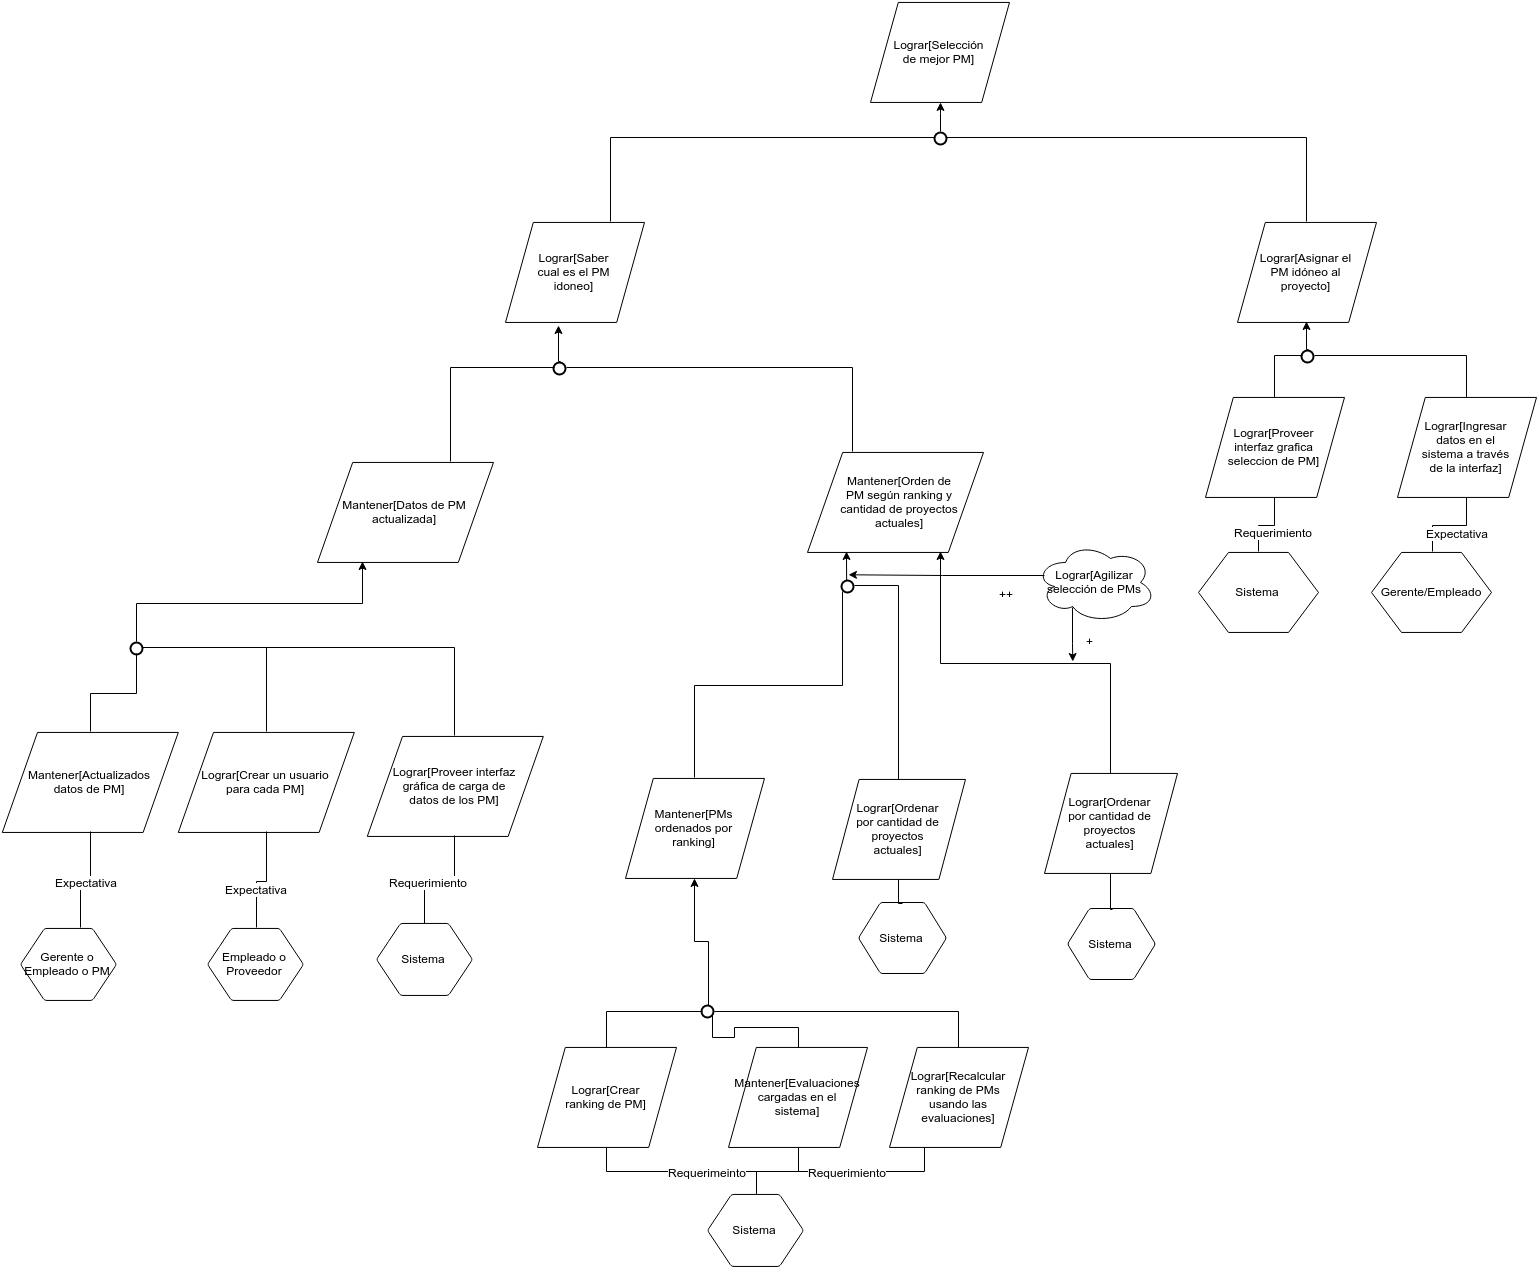
\includegraphics[width=8in, keepaspectratio, angle=90]{imagenes/seleccion.png}
\end{figure}
